%%%%%%%%%%%%%%%%%%%%%%%%%%%%%%%%%%%%%%%%%
% Jacobs Landscape Poster
% LaTeX Template
% Version 1.1 (14/06/14)
%
% Created by:
% Computational Physics and Biophysics Group, Jacobs University
% https://teamwork.jacobs-university.de:8443/confluence/display/CoPandBiG/LaTeX+Poster
% 
% Further modified by:
% Nathaniel Johnston (nathaniel@njohnston.ca)
%
% This template has been downloaded from:
% http://www.LaTeXTemplates.com
%
% License:
% CC BY-NC-SA 3.0 (http://creativecommons.org/licenses/by-nc-sa/3.0/)
%
%%%%%%%%%%%%%%%%%%%%%%%%%%%%%%%%%%%%%%%%%


%----------------------------------------------------------------------------------------
%	PACKAGES AND OTHER DOCUMENT CONFIGURATIONS
%----------------------------------------------------------------------------------------

\documentclass[final]{beamer}

% \usepackage[scale=1.24]{beamerposter} % Use the beamerposter package for laying out the poster
\usepackage[scale=1.075,orientation=portrait]{beamerposter}

\usetheme{confposter} % Use the confposter theme supplied with this template
\usepackage{colortbl}

\definecolor{doe}{RGB}{15, 102, 54}
\definecolor{lbnl-blue}{RGB}{0, 57, 90}
\definecolor{lbnl-teal}{RGB}{0, 118, 129}
\definecolor{lbnl-lg}{RGB}{177, 179, 179}
\definecolor{lbnl-dg}{RGB}{99, 102, 106}

\definecolor{train}{RGB}{179,205,227}
\definecolor{val}{RGB}{254,217,166}

\setbeamercolor{block title}{fg=lbnl-blue,bg=white} % Colors of the block titles
\setbeamercolor{block body}{fg=black,bg=white} % Colors of the body of blocks
\setbeamercolor{block alerted title}{fg=lbnl-blue,bg=lbnl-lg!50} % Colors of the highlighted block titles
\setbeamercolor{block alerted body}{fg=black,bg=lbnl-lg!25} % Colors of the body of highlighted blocks
% Many more colors are available for use in beamerthemeconfposter.sty
\setbeamercolor{titlelike}{bg=lbnl-blue,fg=white}
\setbeamercolor{title}{bg=lbnl-blue,fg=white}

\setbeamercolor{headline}{bg=lbnl-blue,fg=black}
\setbeamercolor{cboxb}{fg=black,bg=lbnl-blue}
\setbeamercolor{cboxr}{fg=black,bg=red}

\usepackage{amsmath}
\DeclareMathOperator*{\argmax}{arg\,max}
\DeclareMathOperator*{\argmin}{arg\,min}

\usepackage{tabu}


%-----------------------------------------------------------
% Define the column widths and overall poster size
% To set effective sepwid, onecolwid and twocolwid values, first choose how many columns you want and how much separation you want between columns
% In this template, the separation width chosen is 0.024 of the paper width and a 4-column layout
% onecolwid should therefore be (1-(# of columns+1)*sepwid)/# of columns e.g. (1-(4+1)*0.024)/4 = 0.22
% Set twocolwid to be (2*onecolwid)+sepwid = 0.464
% Set threecolwid to be (3*onecolwid)+2*sepwid = 0.708

\newlength{\sepwid}
\newlength{\onecolwid}
\newlength{\twocolwid}
\newlength{\threecolwid}
\setlength{\paperwidth}{42in} % A0 width: 46.8in
\setlength{\paperheight}{36in} % A0 height: 33.1in
\setlength{\sepwid}{0.02\paperwidth} % Separation width (white space) between columns
\setlength{\onecolwid}{0.307\paperwidth} % Width of one column
\setlength{\twocolwid}{0.615\paperwidth} % Width of two columns
\setlength{\topmargin}{-1.0in} % Reduce the top margin size
%-----------------------------------------------------------
\usepackage{graphicx}  % Required for including images

\usepackage{booktabs} % Top and bottom rules for tables

\usepackage{mdframed}
\surroundwithmdframed[
    hidealllines=true,
    backgroundcolor=gray!16,
    skipbelow=\baselineskip,
    skipabove=\baselineskip
]{equation}
\surroundwithmdframed[
    hidealllines=true,
    backgroundcolor=gray!16,
    skipbelow=\baselineskip,
    skipabove=\baselineskip
]{align}

% \usefonttheme{professionalfonts} % using non standard fonts for beamer
% \usefonttheme{serif}

% \usepackage[cmintegrals,cmbraces]{newtxmath}
% \usepackage{ebgaramond}
% \usepackage[T1]{fontenc}
% \usepackage{heuristica}
% % \usepackage[heuristica,vvarbb,bigdelims]{newtxmath}
% \usepackage[T1]{fontenc}

\frenchspacing

% \usefonttheme{structurebold}
% \setbeamerfont{headline}{shape=\scshape size=\small}
% \setbeamerfont{subtitle}{size=\scriptsize,series=\bfseries,parent=structure}
% \setbeamerfont{author}{size=\scriptsize,series=\bfseries,parent=structure}
% \setbeamerfont{institute}{size=\scriptsize,series=\bfseries,parent=structure}
% \setbeamerfont{date}{size=\scriptsize,series=\bfseries,parent=structure}

\usepackage[default,regular,black]{sourceserifpro}
\usepackage{newtxmath}
% \usepackage{mathpazo}
% \usepackage[euler-digits,euler-hat-accent]{eulervm}
\usepackage[T1]{fontenc}

% \usepackage{libertine}
% \usepackage{libertinust1math}
% \usepackage[T1]{fontenc}



\newcommand{\train}{\cellcolor{train}Train}
\newcommand{\valdt}{\cellcolor{val}Validation}

\hyphenpenalty=10000
\tolerance=5000

\addtobeamertemplate{headline}{} 
{\begin{tikzpicture}[remember picture, overlay]
     \node [anchor=north west, inner sep=0.875in]  at (current page.north west)
     {
\includegraphics[height=2.04in]{logos/WDE-logo.png}};
  \end{tikzpicture}}
\addtobeamertemplate{headline}{} 
{\begin{tikzpicture}[remember picture, overlay]
     \node [anchor=north east, inner sep=0.875in]  at (current page.north east)
     {
\includegraphics[height=2.04in]{logos/DOE.jpg}};https://v2.overleaf.com/project/5b4d0ff92ca16c5ed63702fe
  \end{tikzpicture}}

%----------------------------------------------------------------------------------------
%	TITLE SECTION 
%----------------------------------------------------------------------------------------

\title{Cross-Validation Methodology in Materials Science} % Poster title

\author{Julien Brenneck\inst{1}, Alexander Dunn\inst{2}, Anubhav Jain\inst{2}} % Author(s)

\institute{\inst{1}University of Massachusetts Amherst, \inst{2}Lawrence Berkeley National Laboratory} % Institution(s)


%----------------------------------------------------------------------------------------

\begin{document}

\addtobeamertemplate{block end}{}{\vspace*{2ex}} % White space under blocks
\addtobeamertemplate{block alerted end}{}{\vspace*{2ex}} % White space under highlighted (alert) blocks

\setlength{\belowcaptionskip}{2ex} % White space under figures
\setlength\belowdisplayshortskip{2ex} % White space under equations

\begin{frame}[t] % The whole poster is enclosed in one beamer frame

\begin{columns}[t] % The whole poster consists of three major columns, the second of which is split into two columns twice - the [t] option aligns each column's content to the top

\begin{column}{\sepwid}\end{column} % Empty spacer column

\begin{column}{\onecolwid} % The first column

%----------------------------------------------------------------------------------------
%	INTRODUCTION
%----------------------------------------------------------------------------------------
% \setstretch{1.}

\begin{alertblock}{Abstract} 
{\small
\quad High-throughput Materials Science has turned towards statistical and machine learning methods in the effort to rapidly accelerate material characterization and discovery.
While these methods promise to take advantage of the accumulating data, without effective quantification of performance and validation methodology there is no assurance that these models will generalize to new data.
% This is especially important in work that is largely comparing the performance of different models on materials data. 
This work highlights potential pitfalls and best practices in the cross-validation of these models.
In particular, it gives practical recommendations for cross-validation methodology.
}
\end{alertblock}

% This work explores the results on cross-validation in the statistical and machine learning literature, and attempts to bring them into material science. 
% Of particular interest is the choice of cross-validation methodology, which has been largely neglected in material science. 

%----------------------------------------------------------------------------------------
%	ESTIMATION OF GENERALIZATION ERROR
%----------------------------------------------------------------------------------------

\begin{block}{Estimation of Generalization Error}

When training a model $\hat f$ on training set $T$, we need to estimate how well it will do on a new set of data $X, Y$.
The \textbf{generalization error} is defined as the expected loss $L$ of the model over any new data, given training set $T$.
\vspace{-0.5em}
\begin{equation}
\text{Err}_T = \mathbf{E}\left[ L(Y, \hat f(X)) \mid T ) \right]
\end{equation}
% \vspace{0.5em}

\begin{itemize}
    \item\textbf{Test error} is average loss over a separate test sample.
    \item\textbf{Training error} is average loss over the training sample. 
\end{itemize}

% \vspace{-0.5em}
% \begin{equation}
% \overline{\text{err}} = {\textstyle \frac{1}{N} \sum_{i=1}^{N} } L\left (Y^{T}_i, \, \hat f( X^{T}_i) \right)
% \end{equation}

% \vspace{0.5em}

Training error does not estimate Err$_T$, and gives over-optimistic results, leading to over-fitting.

\vspace{0.5em}
\begin{figure}
    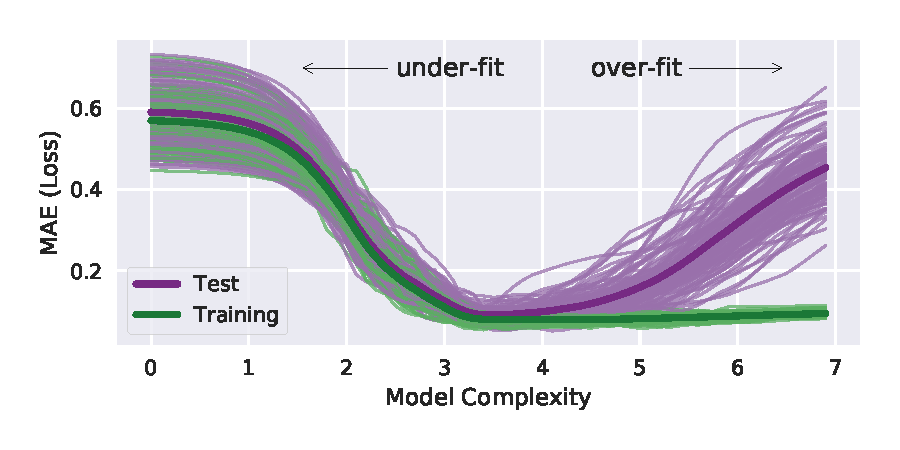
\includegraphics[width=\linewidth]{plots/b-v.pdf}
    \caption{Results of experiment comparing training error and test error as model complexity increases.
    This employed a Support Vector Machine regression on synthetic data, generated from a sinusoidal waveform with Gaussian noise.}
\end{figure}
\vspace{-1.0em}

\begin{itemize}
    \item Do not use training error to estimate model performance.
    \item Use hold-out test sets when possible.
    \item Use cross-validation, Bayesian models, the bootstrap, Bayesian information criterion, ect, for smaller data.
\end{itemize}

% \vspace{0.25em}
% \begin{center}
% \textcolor{lbnl-teal}{\large \bfseries Materials data}
% \end{center}

\end{block}

\vspace{-1.0em}
\begin{block}{Materials Data}
\begin{itemize}
    \item Experimental data is small, often less than 1000 samples. 
    \item Most common materials problems are trying to \textbf{extrapolate} from data instead of \textbf{interpolate}.
    \item Often very high number of features compared to size of the data,  potentially introducing variance. 
\end{itemize}
\end{block}

%----------------------------------------------------------------------------------------

\end{column} % End of the first column

\begin{column}{\sepwid}\end{column} % Empty spacer column

\begin{column}{\onecolwid} % The first column

%----------------------------------------------------------------------------------------
%	CROSS VALIDATION
%----------------------------------------------------------------------------------------

\begin{block}{Cross-Validation}

The \textbf{k-fold} cross-validation (CV) randomly samples the data into $k$ distinct subsets of the same size. 
\vspace{0.5em}
\begin{figure}
    {\footnotesize
    \centering
    \begin{tabu} to 0.75\textwidth{X[0.25,c]|[2pt]X|[2pt]X|[2pt]X|[2pt]X|[2pt]X|[2pt]X[0.1,c]}
    \tabucline{2-6}
    1 & \valdt & \train & \train & \train & \train & \\
    \tabucline{2-6}\noalign{\vskip 0.5em}\tabucline{2-6}
    2 & \train & \valdt & \train & \train & \train & \\
    \tabucline{2-6}\noalign{\vskip 0.5em}\tabucline{2-6}
    3 & \train & \train & \valdt & \train & \train & \\
    \tabucline{2-6}\noalign{\vskip 0.5em}\tabucline{2-6}
    4 & \train & \train & \train & \valdt & \train & \\
    \tabucline{2-6}\noalign{\vskip 0.5em}\tabucline{2-6}
    5 & \train & \train & \train & \train & \valdt & \\
    \tabucline{2-6}
    \end{tabu}
    }
    \vspace{0.75em}
    \caption{5-fold cross-validation. The data is randomly shuffled and then separated into 5 disjoint subsets of the same size, called folds. This gives 5 distinct train/validation splits.}
    \label{fig:folds}
\end{figure}
\vspace{-1.25em}
% \begin{equation}
%     \text{CV} = {\textstyle \frac{1}{k} \sum_{i=1}^k} L_i
% \end{equation}
\begin{itemize}
% \Centering
    \item The $k$ models are fit, each using a distinct validation set.
    \item Average of the $k$ validation scores is taken.
\end{itemize}
% Then $k$ models are fit, using the $k$ subsets as a hold out validation set for each, and the average score is taken. 

\end{block}
\vspace{-0.75em}

%----------------------------------------------------------------------------------------
%	VARIANCE OF CV
%----------------------------------------------------------------------------------------


\begin{block}{Variance of the k-Fold Cross-Validation}
% \vspace{-0.25em}
\begin{center}
\textcolor{lbnl-teal}{\bfseries How does the choice of k affect the result?}
\end{center}
\vspace{-0.25em}
\begin{figure}
    \centering
    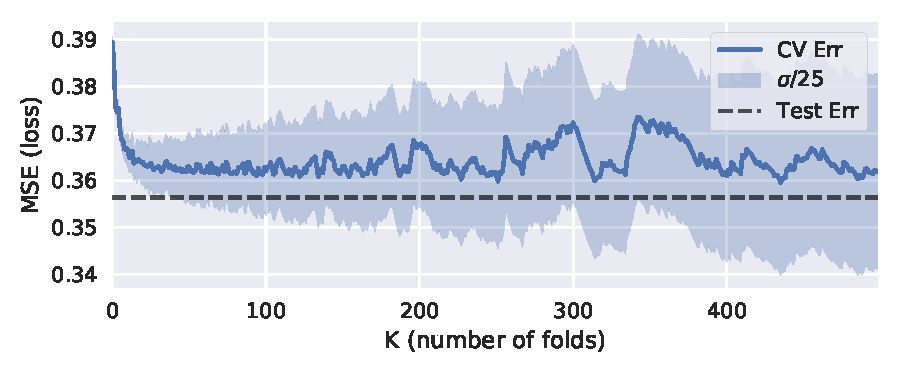
\includegraphics[width=\linewidth]{plots/kfold-cv-std-6x3.pdf}
    \caption{Computational experiment showing the sample mean and standard deviation of the $k$-fold scores for increasing values of $k$. This employed a Support Vector Regression (SVR) using a Radial Basis Function (RBF) kernel on synthetic data, with Mean Squared Error (MSE) loss.}
    \label{fig:cv-var}
\end{figure}
\vspace{-0.5em}
This highlights part of the bias-variance trade-off.
\begin{itemize}
    \item Small $k$ gives higher bias, lower variance in CV estimate.
    \item Larger $k$ gives lower bias, higher variance in CV estimate.
    \item Larger $k$ much more computationally expensive!
    \item In general, \textcolor{lbnl-teal}{\bfseries k=5 or k=10} is a practical compromise. 
\end{itemize}
\vspace{0.25em}
 When $k=N$ we get  \textbf{Leave One Out CV} (LOOCV). 
For some models LOOCV has low variance and can be computed efficiently, but in general can have high variance and is computationally expensive.

\vspace{1.0em}

There is \textbf{no unbiased estimator} for $k$-fold CV variance.
\begin{itemize}
    \item Bias can be same order of magnitude as total variance.
    \item Conservative estimates of CV variance difficult in practice.
    \item Robust comparisons of model performance difficult to make, as confidence intervals require variance estimates.
\end{itemize}

\vspace{0.5em}

\textbf{Repeated k-fold} reduces variance of the CV estimate, without affecting bias. 
Recommended when computationally feasible. 
Repeats $k$-fold CV with new random folds and averages the scores.
\end{block}





%----------------------------------------------------------------------------------------

\end{column} % End of the first column

\begin{column}{\sepwid}\end{column} % Empty spacer column

\begin{column}{\onecolwid} % The third column

%----------------------------------------------------------------------------------------
%	MODEL SELECTION & EVALUATION
%----------------------------------------------------------------------------------------

\begin{block}{Model Selection for Materials Data}

The process of model selection, choosing a model and hyper-parameters, can heavily bias estimated model performance without proper methodology. 
% A pitfall in materials is in feature selection, which needs to be considered as part of model selection.
% The large number of features in materials data can increase this bias. 
\begin{itemize}
    % \item Materials data sets often small with large numbers of features.
    \item Feature selection can introduce bias, with more features making the effect worse, a concern for materials data.
    \item Feature selection needs to be a part of model selection.
\end{itemize}
An experiment was conducted using materials data to show the susceptibility to over-fitting in model selection.
% \vspace{-0.5em}
\begin{table}[ht]
  \begin{minipage}[b]{0.6\textwidth}
    \Centering
    \small
    \taburulecolor{lbnl-dg}{
    \tabulinesep=0.5em
    % \vspace{-3em}
    \begin{tabu} to \textwidth{X[4] X[4,r] X[4,r] X[4,r] X[4,r]}
    \toprule
    Model  & Train Err & 10-fold CV Err & Nested CV Err & Test Err \\
    \midrule
    KRR  & \textcolor{BrickRed}{\bfseries 10.17} & \textcolor{BurntOrange}{\bfseries 18.26} & \textcolor{NavyBlue!50!gray}{\bfseries 21.41} &  \textcolor{doe}{\bfseries 21.61}   \\
    GBTR & \textcolor{BrickRed}{\bfseries  3.37} & \textcolor{BurntOrange}{\bfseries 14.37} & \textcolor{NavyBlue!50!gray}{\bfseries 16.38} & \textcolor{doe}{\bfseries 20.90}   \\
    GPR  & \textcolor{BrickRed}{\bfseries  0.00} & \textcolor{BurntOrange}{\bfseries 32.63} & \textcolor{NavyBlue!50!gray}{\bfseries 33.96} & \textcolor{doe}{\bfseries 35.45}   \\
    \bottomrule
    \end{tabu}
    \vspace{2.25em}
    }
    \end{minipage}
  \begin{minipage}[b]{0.39\textwidth}
    \centering
    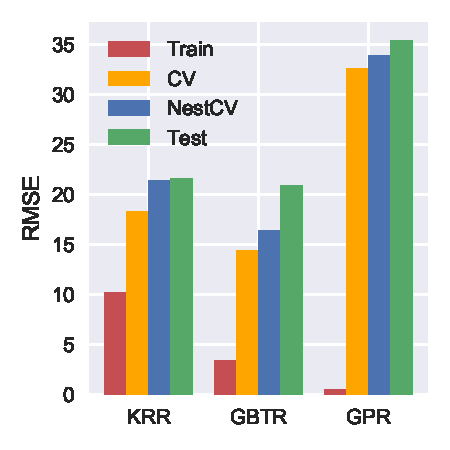
\includegraphics[width=0.98\textwidth]{plots/errors-3x3.pdf}
  \end{minipage}
    \label{tbl:overfit}
    \vspace{-2em}
    \caption{Comparing prediction errors of an over-fit model.
    Model selection CV estimates can seriously underestimate true test error.
    Predicting bulk modulus based on 140 compositional and structural features, from matminer's ElementProperty and density featurizers, with a Kernel Ridge Regression (KRR), Gradient Boosted Tree Regression (GBTR), and a Gaussian Process Regression (GPR). Error is RMSE in GPa. }
\end{table}

\vspace{-1em}

\begin{itemize}
    \item Use a hold out test set for model selection.
    \item Consider nested CV or Bayesian methodology for small data.
    \item Over-fitting in model selection is a problem in practice, and can cause over or under fitting in the final model.
    \item Feature selection can cause bias if not part of cross-validation.
\end{itemize}

\vspace{0.25em}

Bias is less important than variance in model selection (assuming a constant bias) as the "best" model will still be chosen. 
% Thus $k=5$ may be a better choice in model selection.
% to trade some variance for bias and reduce the computational cost.
\end{block}

\vspace{-0.25em}

%----------------------------------------------------------------------------------------
%	CONCLUSION
%----------------------------------------------------------------------------------------


\begin{block}{Conclusion}

\begin{itemize}
    \item Use a validation set or $k$-fold CV with $k=5$ or $k=10$ depending on size of data, and avoid LOOCV (in general).
    \item Use repeated k-fold CV to increase confidence in CV estimate.
    \item Model selection and feature selection need to be internal to validation scheme to avoid over-fitting.
    \item A good methodology is using a test / train split, then using CV for model selection on the training data, and measuring final model performance on the test data.
\end{itemize}


\end{block}

\vspace{-0.5em}

%----------------------------------------------------------------------------------------
%	ACKNOWLEDGEMENTS
%----------------------------------------------------------------------------------------

\begin{alertblock}{Acknowledgements}
\small 
This work was supported in part by the U.S. Department of Energy, Office of Science, Office of Workforce Development for Teachers and Scientists (WDTS) under the Science Undergraduate Laboratory Internship (SULI) program.
Additional funding was provided by the U.S. Department of Energy, Office of Basic Energy Sciences, Early Career Research Program.
\end{alertblock}


%----------------------------------------------------------------------------------------
%	CONTACT INFORMATION
%----------------------------------------------------------------------------------------

% \setbeamercolor{block alerted title}{fg=black,bg=norange} % Change the alert block title colors
% \setbeamercolor{block alerted body}{fg=black,bg=white} % Change the alert block body colors

% \begin{alertblock}{Contact Information}

% \begin{center}
% jbrenneck@umass.edu
% \end{center}

% \end{alertblock}

%----------------------------------------------------------------------------------------

\end{column} % End of the third column

\end{columns} % End of all the columns in the poster

\end{frame} % End of the enclosing frame

\end{document}
